% Page budget: at most 7 pages.
\section{Dynamic solution and canonical optimization model}\label{sec:control}

The resource problems in Sections~4--5 take productive library values as
inputs.  This section closes the model by solving those values from the same
raw admission and update laws used to define the sufficient state.  It then
places exact safe compression, hard capacity, resource pricing, and elasticity
on one six-state rational benchmark.  Exact arithmetic comes first throughout;
\texttt{Float64} is used only for the final numerical diagnostic.

\subsection{Unified Bellman operator}

Write \(K=K_L=(F_L,C_L)\), let \(A(K)\) be the finite feasible project menu,
and let \(d(q)>0\) be the duration of project \(q\).  Conditional on \(B_0=b\),
the belief-path marginal during research is
\begin{equation}\label{eq:control-belief-path}
 \Pr(B_{0:d(q)}=b_{0:d(q)}\mid b)
 =\mathbf 1\{b_0=b\}\prod_{t=0}^{d(q)-1}P_B(b_t,b_{t+1}).
\end{equation}
Let \(\Lambda_q(\cdot\mid b,K)\) be the exact joint law of this path and the
admitted outcome \(O\); path and admission need not be independent.  During
research, incumbent operation contributes
\begin{equation}\label{eq:control-operating-reward}
 \mathcal O_q(B_{0:d(q)-1};K)
 :=\sum_{t=0}^{d(q)-1}\beta^t
   \mathbf 1\{o(q)=1\}F_K(B_t).
\end{equation}

\begin{definition}[Unified Continue, research, and Bellman operators]
\label{def:dynamic-control-operators}
For \(V:B\times\mathcal K_{\rm real}\to\mathbb R\), define
\begin{align}
 (\mathsf C V)(b,K)
   &:=F_K(b)+\beta\sum_{b'}P_B(b,b')V(b',K),
   \label{eq:control-continue}\\
 (\mathsf R_qV)(b,K)
   &:=-\kappa(b,K,q)
     +\mathbb E_{\Lambda_q(\cdot\mid b,K)}\!\left[
       \mathcal O_q(B_{0:d(q)-1};K)
       +\beta^{d(q)}V\!\left(B_{d(q)},
          \operatorname{addK}(K,O)\right)\right],
   \label{eq:control-research}\\
 (\mathsf TV)(b,K)
   &:=\max\!\left\{(\mathsf CV)(b,K),
       \max_{q\in A(K)}(\mathsf R_qV)(b,K)\right\}.
 \label{eq:control-bellman-operator}
\end{align}
If \(A(K)=\varnothing\), the inner research maximum is omitted, so
\((\mathsf TV)(b,K)=(\mathsf CV)(b,K)\).
\end{definition}

Continue consumes one date; research consumes \(d(q)\) dates.  Suspending
operation removes the block in \eqref{eq:control-operating-reward}, not belief
evolution or the terminal raw update.  At a finite horizon only projects whose
duration fits the remaining dates are feasible.  The stationary equation is
\(V_\infty=\mathsf TV_\infty\) on the complete menu.

\begin{proposition}[Finite-state contraction and selectors]
\label{prop:finite-horizon-action-attainment}
\label{thm:finite-state-contraction}
Suppose all carriers are finite, primitive probabilities and payoffs are exact
rationals, project durations are positive, and \(0\le\beta<1\).  Every
finite-horizon Bellman maximum is attained.  The raw and compressed stationary
operators are monotone sup-norm contractions with modulus \(\beta\), have
unique fixed points, and agree under raw-to-compressed projection.  Hence
dynamically innovation-equivalent libraries have equal finite- and
infinite-horizon values.  A stationary maximizing selector exists, satisfies
\(\mathsf T_{\pi^\star}V_\infty=V_\infty=V^{\pi^\star}\), and lifts to a raw
stationary selector.  For any initial table \(v_0\),
\begin{equation}\label{eq:control-geometric-bound}
 \lVert\mathsf T^n v_0-V_\infty\rVert_\infty
 \le \frac{\lVert v_0-\mathsf T v_0\rVert_\infty\beta^n}{1-\beta}.
\end{equation}
\end{proposition}

The contraction, intertwining, and selector argument is in
\cref{app:di-quotient}.  Appendix~D gives the numerical stopping rule and
compact verification certificate; Online Supplement~S4 retains the complete
convergence history.

\subsection{Unified six-state compressed benchmark}
\label{sec:numerics}

The benchmark is constructed from raw primitives.  Its catalog is
\[
\begin{array}{c|c|c|l}
s&(j_s(\ell),j_s(h))&\operatorname{mods}(s)&\text{role}\\ \hline
s_0&(0,0)&\varnothing&\text{mandatory inactive policy}\\
c_A&(0,0)&\{m\}&\text{silent carrier A}\\
c_B&(0,0)&\{m\}&\text{silent carrier B}\\
g&(2,4)&\{m\}&\text{profitable descendant and carrier}.
\end{array}
\]
Closure is the identity on \(\{m\}\), and every raw library contains \(s_0\).
Exhausting the eight subsets of \(\{c_A,c_B,g\}\) produces three compressed
library states,
\[
 K_0=((0,0),\varnothing),\qquad
 K_1=((0,0),\{m\}),\qquad
 K_2=((2,4),\{m\}).
\]
Together with \(B=\{\ell,h\}\), these are the six Bellman states.  The exact
belief law and discount are
\begin{equation}\label{eq:canonical-belief-kernel}
 P_B=\begin{pmatrix}3/4&1/4\\[2pt]1/4&3/4\end{pmatrix},\qquad
 P_B^2=\begin{pmatrix}5/8&3/8\\[2pt]3/8&5/8\end{pmatrix},\qquad
 \beta=1/2.
\end{equation}

Discover is available at \(K_0\), lasts one date, operates the incumbent, and
costs \(1/32\) at \(\ell\) and \(1\) at \(h\).  Raw generation and verification
give
\(\Gamma_D=\tfrac14\delta_\bot+\tfrac12\delta_{c_A}
 +\tfrac14\delta_{c_B}\).
Scale is available at \(K_1,K_2\), lasts two dates, operates the incumbent,
costs \(3/16\), and admits \(g\) with marginal probability \(3/4\).  Its
success is correlated with the terminal belief: the exact conditional
probability is \(3/5\) for \((B_0,B_2)=(\ell,\ell)\), \(1/3\) for
\((h,\ell)\), and \(1\) when \(B_2=h\).  Applying the raw update
\(L\oplus s=L\cup\{s\}\) and only then projecting gives
\[
 R_D(K_0)=\tfrac14\delta_{K_0}+\tfrac34\delta_{K_1},\qquad
 R_S(K_1)=\tfrac14\delta_{K_1}+\tfrac34\delta_{K_2},\qquad
 R_S(K_2)=\delta_{K_2}.
\]
Thus no transition is stipulated directly on the compressed carrier.  The
full path-by-admission atoms and reward-block algebra are in Online
Supplement~S4.

\begin{figure}[htbp]
  \centering
  % Generated by julia/scripts/solve_unified_canonical_benchmark.jl.
% Source: experiments/results/summaries/unified_canonical_transition_edges.csv.
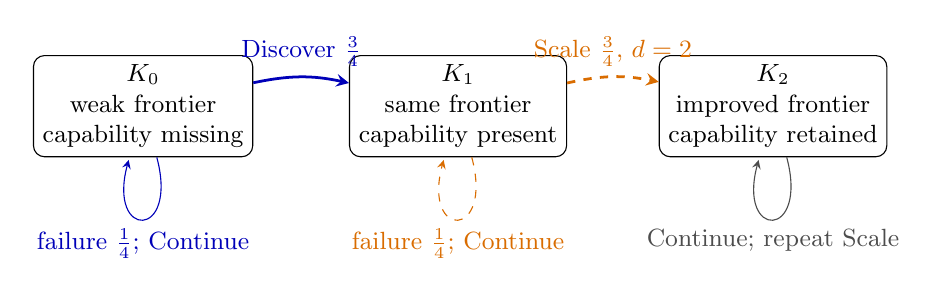
\begin{tikzpicture}[>=stealth,font=\small]
  \node[draw,rounded corners,align=center,minimum width=2.3cm] (k0) at (0,0)
    {\(K_0\)\\weak frontier\\capability missing};
  \node[draw,rounded corners,align=center,minimum width=2.3cm] (k1) at (4,0)
    {\(K_1\)\\same frontier\\capability present};
  \node[draw,rounded corners,align=center,minimum width=2.3cm] (k2) at (8,0)
    {\(K_2\)\\improved frontier\\capability retained};
  \draw[->,blue!72!black,line width=1.0pt]
    (k0) to[bend left=12] node[above] {Discover \(\frac{3}{4}\)} (k1);
  \draw[->,orange!85!black,dashed,line width=1.0pt]
    (k1) to[bend left=12] node[above] {Scale \(\frac{3}{4}\), \(d=2\)} (k2);
  \draw[->,blue!72!black]
    (k0) edge[loop below] node {failure \(\frac{1}{4}\); Continue} (k0);
  \draw[->,orange!85!black,dashed]
    (k1) edge[loop below] node {failure \(\frac{1}{4}\); Continue} (k1);
  \draw[->,black!70]
    (k2) edge[loop below] node {Continue; repeat Scale} (k2);
\end{tikzpicture}

  \caption{Exact raw-derived compressed transition law.  Each edge label is
  the one-project probability obtained by applying raw generation,
  verification, admission, and library update before projection.  Solid blue
  is Discover, dashed orange is Scale, and self-loops collect failure and
  Continue; no intermediate states or smooth interpolation are implied.}
  \label{fig:canonical-compressed-transition}
\end{figure}

\subsection{Exact rational dynamic solution}

Exact raw and compressed policy iteration terminate after three improvement
steps with policy-equation and Bellman residuals equal to zero.  Projection
matches values and actions on all eight raw libraries.  The minimum exact
winning margin is \(3/16\), so the benchmark has no action tie.

\begin{table}[htbp]
\centering
\small
% Generated by julia/scripts/generate_main_text_tables.jl.
% Exact source: experiments/results/summaries/unified_canonical_resource_channel_elasticities.csv.
\begin{tabular}{@{}llrll@{}}
\toprule
State & Belief & \(V^\star\) (payoff units) & \(\pi^\star\) & Winning margin (payoff units) \\
\midrule
\(K_{0}\)&\(\ell\)&\(\frac{115}{288}\)&Discover&\(\frac{23}{96}\)\\
\(K_{0}\)&\(h\)&\(\frac{23}{288}\)&Continue&\(\frac{245}{384}\)\\
\(K_{1}\)&\(\ell\)&\(1\)&Scale&\(\frac{23}{48}\)\\
\(K_{1}\)&\(h\)&\(\frac{7}{6}\)&Scale&\(\frac{29}{48}\)\\
\(K_{2}\)&\(\ell\)&\(\frac{14}{3}\)&Continue&\(\frac{3}{16}\)\\
\(K_{2}\)&\(h\)&\(\frac{22}{3}\)&Continue&\(\frac{3}{16}\)\\
\bottomrule
\end{tabular}

\caption{Exact rational stationary solution of the raw-derived six-state
benchmark.  Values and winning margins are measured in the benchmark's payoff
units.  Denominator-one rationals are rendered as integers.  Appendix~D
reports the zero-residual certificate; Online Supplement~S4 reports the full
action-value record.}
\label{tab:canonical-exact-solution}
\end{table}

\subsection{Resource weights and exact safe-compression solutions}

Write \(I,A,B,D\) for \(s_0,c_A,c_B,g\).  The three prospectively fixed
integer schedules keep the silent carriers symmetric.  In the coordinate
order \((I,A,B,D)\), their exact weight vectors are equal-active
\((1,1,1,1)\), carrier-heavy \((1,2,2,1)\), and descendant-heavy
\((1,1,1,2)\).
The positive mandatory weight is common to every feasible library.  It shifts
reported capacities and penalized levels but not within-schedule switching
prices.

Complete enumeration shows that the full source compresses uniquely to
\(I+D\) under every
schedule, keeps frontier \((2,4)\) and closure \(\{m\}\), and saves one-half,
two-thirds, or two-fifths of source burden.  These are exact finite
enumeration certificates, not consequences of a greedy rule.  The complete
source-by-source correspondence and exact burden reductions are in Online
Supplement~S4.

\subsection{Capacity-optimal library path}

The hard-capacity optimizer is evaluated at every attainable burden.  Equal
active and carrier heavy jump directly from \(I\) to \(I+D\).  Descendant
heavy passes through the tied carrier pair \(I+A\) or \(I+B\); the resulting
capacity complements make the second value increment exceed the first.
The exact paths, globally active positive switch prices, and inactive pairwise
crossing candidates are tabulated in Online Supplement~S4; the main text uses
the combined economic-geometry figure to avoid repeating the same staircase
and breakpoints.

\subsection{Penalized envelope, breakpoints, and selected burden}

For each schedule and belief, the penalized problem exhausts the eight affine
branches \(V(b,L)-\lambda W(L)\).  Only \(I+D\) and \(I\) are globally active
for \(\lambda>0\).  Equal active and carrier heavy switch at \(1229/288\)
from low belief and \(2089/288\) from high belief.  Descendant heavy doubles
the relevant burden difference, so its breakpoints are \(1229/576\) and
\(2089/576\).  At a breakpoint both libraries are optimal; away from it the
optimizer is unique after removal of redundant equal-state libraries.

\subsection{Innovation duration and elasticity values}

At \(\beta=1/2\), the exact local fixed-policy discount elasticities
\(D_\beta=\beta V_\beta/V\) are
\[
\begin{array}{c|cc|l}
 &\ell&h&\text{productive channel}\\ \hline
I&10777/2070&14089/2070&\text{generative}\\
I{+}A\text{ or }I{+}B&56/15&53/15&\text{generative}\\
I{+}D&25/21&29/33&\text{operational}.
\end{array}
\]
The zero complementary channel is reported as a zero contribution, not with
an elasticity.  In the registered bridge calculation with gross descendant
value one, duration three, and normalized positive margin \(1/16\), the exact
discount/survival, admission/payoff, and cost elasticities are respectively
\(48\), \(16\), and \(-15\).  These are fixed-exposure values; they do not
differentiate through a library or action switch.

\subsection{Floating-Point Verification}

After fixing the exact solution and optimizer correspondences, the same
raw-law model's \texttt{Float64} value iteration stops after 42 steps.  Its
final increment is \(5.5422\times10^{-13}\), its Bellman residual is
\(2.7711\times10^{-13}\), and its Float64 a-posteriori contraction bound is
\(5.5422\times10^{-13}\).  Converting the binary Float64 iterate exactly to
rationals gives maximum error \(5.5482\times10^{-13}\) against the exact
rational table, below the exactly re-evaluated residual-based certificate
\(5.5489\times10^{-13}\).  The six actions match
\cref{tab:canonical-exact-solution}.  Appendix~D reports the stopping rule and
compact certificate, while Online Supplement~S4 reports the complete history;
the policy-map response remains with the controlled diagnostics in
Online Supplement~S5.

\begin{figure}[p]
  \centering
  % Generated by julia/scripts/generate_figure_audit_artifacts.jl.
% Exact sources: unified_elasticity_switching_v1_{capacity,penalized_path}.csv.
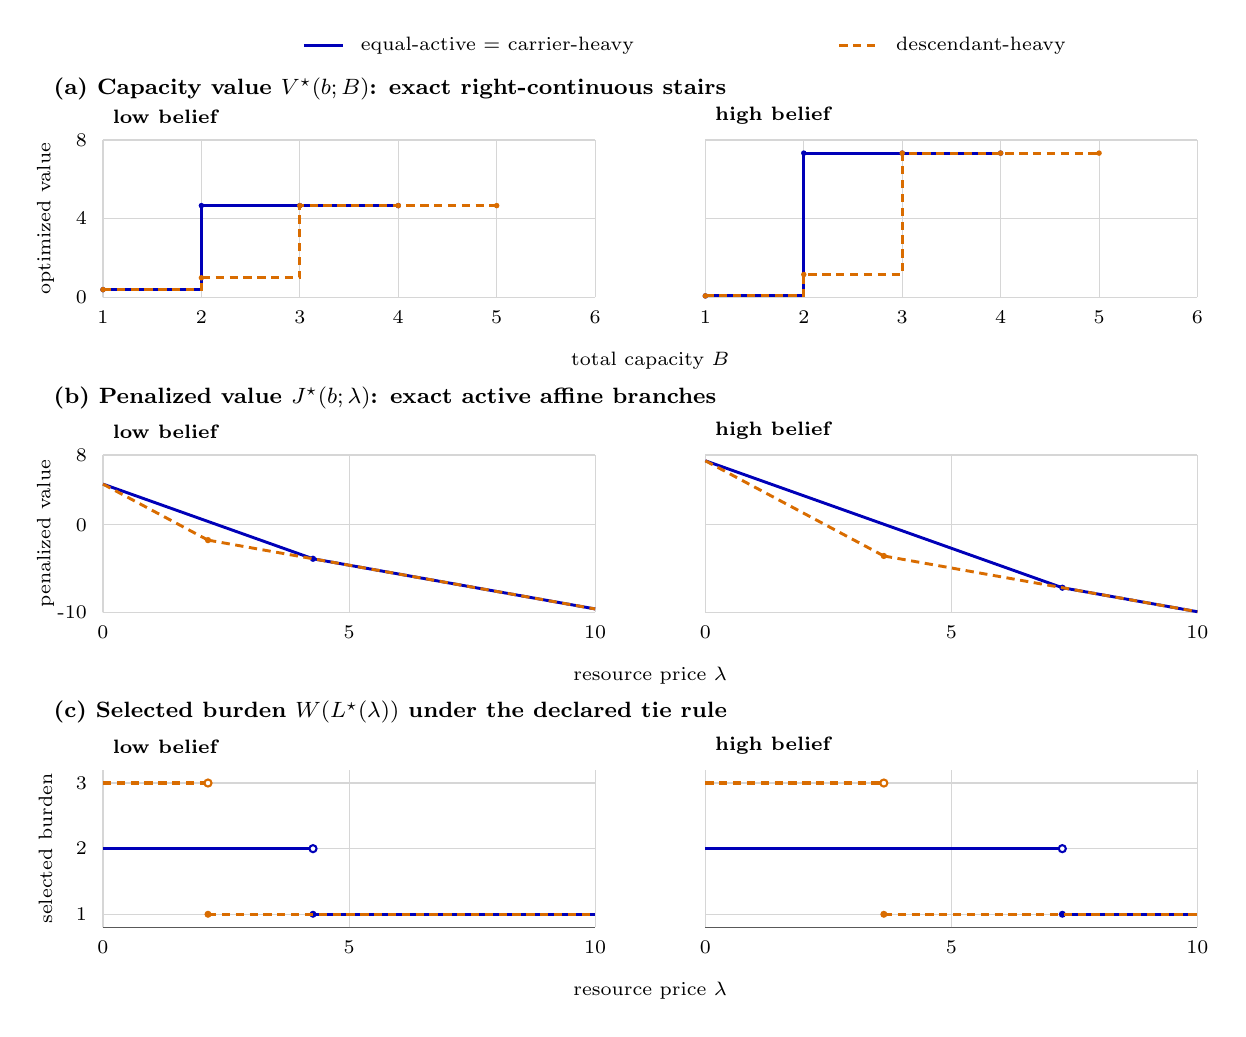
\begin{tikzpicture}[x=1cm,y=1cm,font=\scriptsize]
  \draw[blue!72!black,line width=1.05pt] (3.55,10.95) -- (4.05,10.95);
  \node[anchor=west] at (4.15,10.95) {equal-active = carrier-heavy};
  \draw[orange!85!black,densely dashed,line width=1.05pt] (10.35,10.95) -- (10.85,10.95);
  \node[anchor=west] at (10.95,10.95) {descendant-heavy};
  \node[font=\bfseries\footnotesize,anchor=west] at (0.25,10.40) {(a) Capacity value \(V^\star(b;B)\): exact right-continuous stairs};
  \node[font=\bfseries\scriptsize,anchor=south west] at (1.0,9.83) {low belief};
  \draw[black!65] (1.0,7.75) -- (7.25,7.75);
  \draw[black!65] (1.0,7.75) -- (1.0,9.75);
  \draw[black!16] (1.0,7.75) -- (1.0,9.75);
  \node[anchor=north,font=\scriptsize] at (1.0,7.7) {1};
  \draw[black!16] (2.25,7.75) -- (2.25,9.75);
  \node[anchor=north,font=\scriptsize] at (2.25,7.7) {2};
  \draw[black!16] (3.5,7.75) -- (3.5,9.75);
  \node[anchor=north,font=\scriptsize] at (3.5,7.7) {3};
  \draw[black!16] (4.75,7.75) -- (4.75,9.75);
  \node[anchor=north,font=\scriptsize] at (4.75,7.7) {4};
  \draw[black!16] (6.0,7.75) -- (6.0,9.75);
  \node[anchor=north,font=\scriptsize] at (6.0,7.7) {5};
  \draw[black!16] (7.25,7.75) -- (7.25,9.75);
  \node[anchor=north,font=\scriptsize] at (7.25,7.7) {6};
  \draw[black!16] (1.0,7.75) -- (7.25,7.75);
  \node[anchor=east,font=\scriptsize] at (0.92,7.75) {0};
  \draw[black!16] (1.0,8.75) -- (7.25,8.75);
  \node[anchor=east,font=\scriptsize] at (0.92,8.75) {4};
  \draw[black!16] (1.0,9.75) -- (7.25,9.75);
  \node[anchor=east,font=\scriptsize] at (0.92,9.75) {8};
  \draw[blue!72!black,solid,line width=1.05pt] (1.0,7.84983) -- (2.25,7.84983) -- (2.25,8.91667) -- (3.5,8.91667) -- (3.5,8.91667) -- (4.75,8.91667) -- (4.75,8.91667);
  \fill[blue!72!black] (1.0,7.84983) circle (0.035);
  \fill[blue!72!black] (2.25,8.91667) circle (0.035);
  \fill[blue!72!black] (3.5,8.91667) circle (0.035);
  \fill[blue!72!black] (4.75,8.91667) circle (0.035);
  \draw[orange!85!black,densely dashed,line width=1.05pt] (1.0,7.84983) -- (2.25,7.84983) -- (2.25,8.0) -- (3.5,8.0) -- (3.5,8.91667) -- (4.75,8.91667) -- (4.75,8.91667) -- (6.0,8.91667) -- (6.0,8.91667);
  \fill[orange!85!black] (1.0,7.84983) circle (0.035);
  \fill[orange!85!black] (2.25,8.0) circle (0.035);
  \fill[orange!85!black] (3.5,8.91667) circle (0.035);
  \fill[orange!85!black] (4.75,8.91667) circle (0.035);
  \fill[orange!85!black] (6.0,8.91667) circle (0.035);
  \node[font=\bfseries\scriptsize,anchor=south west] at (8.65,9.83) {high belief};
  \draw[black!65] (8.65,7.75) -- (14.9,7.75);
  \draw[black!65] (8.65,7.75) -- (8.65,9.75);
  \draw[black!16] (8.65,7.75) -- (8.65,9.75);
  \node[anchor=north,font=\scriptsize] at (8.65,7.7) {1};
  \draw[black!16] (9.9,7.75) -- (9.9,9.75);
  \node[anchor=north,font=\scriptsize] at (9.9,7.7) {2};
  \draw[black!16] (11.15,7.75) -- (11.15,9.75);
  \node[anchor=north,font=\scriptsize] at (11.15,7.7) {3};
  \draw[black!16] (12.4,7.75) -- (12.4,9.75);
  \node[anchor=north,font=\scriptsize] at (12.4,7.7) {4};
  \draw[black!16] (13.65,7.75) -- (13.65,9.75);
  \node[anchor=north,font=\scriptsize] at (13.65,7.7) {5};
  \draw[black!16] (14.9,7.75) -- (14.9,9.75);
  \node[anchor=north,font=\scriptsize] at (14.9,7.7) {6};
  \draw[black!16] (8.65,7.75) -- (14.9,7.75);
  \draw[black!16] (8.65,8.75) -- (14.9,8.75);
  \draw[black!16] (8.65,9.75) -- (14.9,9.75);
  \draw[blue!72!black,solid,line width=1.05pt] (8.65,7.76997) -- (9.9,7.76997) -- (9.9,9.58333) -- (11.15,9.58333) -- (11.15,9.58333) -- (12.4,9.58333) -- (12.4,9.58333);
  \fill[blue!72!black] (8.65,7.76997) circle (0.035);
  \fill[blue!72!black] (9.9,9.58333) circle (0.035);
  \fill[blue!72!black] (11.15,9.58333) circle (0.035);
  \fill[blue!72!black] (12.4,9.58333) circle (0.035);
  \draw[orange!85!black,densely dashed,line width=1.05pt] (8.65,7.76997) -- (9.9,7.76997) -- (9.9,8.04167) -- (11.15,8.04167) -- (11.15,9.58333) -- (12.4,9.58333) -- (12.4,9.58333) -- (13.65,9.58333) -- (13.65,9.58333);
  \fill[orange!85!black] (8.65,7.76997) circle (0.035);
  \fill[orange!85!black] (9.9,8.04167) circle (0.035);
  \fill[orange!85!black] (11.15,9.58333) circle (0.035);
  \fill[orange!85!black] (12.4,9.58333) circle (0.035);
  \fill[orange!85!black] (13.65,9.58333) circle (0.035);
  \node[anchor=north] at (7.95,7.18) {total capacity \(B\)};
  \node[rotate=90] at (0.27,8.75) {optimized value};
  \node[font=\bfseries\footnotesize,anchor=west] at (0.25,6.48) {(b) Penalized value \(J^\star(b;\lambda)\): exact active affine branches};
  \node[font=\bfseries\scriptsize,anchor=south west] at (1.0,5.83) {low belief};
  \draw[black!65] (1.0,3.75) -- (7.25,3.75);
  \draw[black!65] (1.0,3.75) -- (1.0,5.75);
  \draw[black!16] (1.0,3.75) -- (1.0,5.75);
  \node[anchor=north,font=\scriptsize] at (1.0,3.7) {0};
  \draw[black!16] (4.125,3.75) -- (4.125,5.75);
  \node[anchor=north,font=\scriptsize] at (4.125,3.7) {5};
  \draw[black!16] (7.25,3.75) -- (7.25,5.75);
  \node[anchor=north,font=\scriptsize] at (7.25,3.7) {10};
  \draw[black!16] (1.0,3.75) -- (7.25,3.75);
  \node[anchor=east,font=\scriptsize] at (0.92,3.75) {-10};
  \draw[black!16] (1.0,4.86111) -- (7.25,4.86111);
  \node[anchor=east,font=\scriptsize] at (0.92,4.86111) {0};
  \draw[black!16] (1.0,5.75) -- (7.25,5.75);
  \node[anchor=east,font=\scriptsize] at (0.92,5.75) {8};
  \draw[blue!72!black,solid,line width=1.05pt] (1.0,5.37963) -- (3.6671,4.43133);
  \draw[blue!72!black,solid,line width=1.05pt] (3.6671,4.43133) -- (7.25,3.79437);
  \fill[blue!72!black] (3.6671,4.43133) circle (0.04);
  \draw[orange!85!black,densely dashed,line width=1.05pt] (1.0,5.37963) -- (2.33355,4.6684);
  \draw[orange!85!black,densely dashed,line width=1.05pt] (2.33355,4.6684) -- (7.25,3.79437);
  \fill[orange!85!black] (2.33355,4.6684) circle (0.04);
  \node[font=\bfseries\scriptsize,anchor=south west] at (8.65,5.83) {high belief};
  \draw[black!65] (8.65,3.75) -- (14.9,3.75);
  \draw[black!65] (8.65,3.75) -- (8.65,5.75);
  \draw[black!16] (8.65,3.75) -- (8.65,5.75);
  \node[anchor=north,font=\scriptsize] at (8.65,3.7) {0};
  \draw[black!16] (11.775,3.75) -- (11.775,5.75);
  \node[anchor=north,font=\scriptsize] at (11.775,3.7) {5};
  \draw[black!16] (14.9,3.75) -- (14.9,5.75);
  \node[anchor=north,font=\scriptsize] at (14.9,3.7) {10};
  \draw[black!16] (8.65,3.75) -- (14.9,3.75);
  \draw[black!16] (8.65,4.86111) -- (14.9,4.86111);
  \draw[black!16] (8.65,5.75) -- (14.9,5.75);
  \draw[blue!72!black,solid,line width=1.05pt] (8.65,5.67593) -- (13.18342,4.06404);
  \draw[blue!72!black,solid,line width=1.05pt] (13.18342,4.06404) -- (14.9,3.75887);
  \fill[blue!72!black] (13.18342,4.06404) circle (0.04);
  \draw[orange!85!black,densely dashed,line width=1.05pt] (8.65,5.67593) -- (10.91671,4.46701);
  \draw[orange!85!black,densely dashed,line width=1.05pt] (10.91671,4.46701) -- (14.9,3.75887);
  \fill[orange!85!black] (10.91671,4.46701) circle (0.04);
  \node[anchor=north] at (7.95,3.18) {resource price \(\lambda\)};
  \node[rotate=90] at (0.27,4.75) {penalized value};
  \node[font=\bfseries\footnotesize,anchor=west] at (0.25,2.48) {(c) Selected burden \(W(L^\star(\lambda))\) under the declared tie rule};
  \node[font=\bfseries\scriptsize,anchor=south west] at (1.0,1.83) {low belief};
  \draw[black!65] (1.0,-0.25) -- (7.25,-0.25);
  \draw[black!65] (1.0,-0.25) -- (1.0,1.75);
  \draw[black!16] (1.0,-0.25) -- (1.0,1.75);
  \node[anchor=north,font=\scriptsize] at (1.0,-0.3) {0};
  \draw[black!16] (4.125,-0.25) -- (4.125,1.75);
  \node[anchor=north,font=\scriptsize] at (4.125,-0.3) {5};
  \draw[black!16] (7.25,-0.25) -- (7.25,1.75);
  \node[anchor=north,font=\scriptsize] at (7.25,-0.3) {10};
  \draw[black!16] (1.0,-0.08333) -- (7.25,-0.08333);
  \node[anchor=east,font=\scriptsize] at (0.92,-0.08333) {1};
  \draw[black!16] (1.0,0.75) -- (7.25,0.75);
  \node[anchor=east,font=\scriptsize] at (0.92,0.75) {2};
  \draw[black!16] (1.0,1.58333) -- (7.25,1.58333);
  \node[anchor=east,font=\scriptsize] at (0.92,1.58333) {3};
  \draw[blue!72!black,solid,line width=1.15pt] (1.0,0.75) -- (3.6671,0.75);
  \draw[blue!72!black,solid,line width=1.15pt] (3.6671,-0.08333) -- (7.25,-0.08333);
  \draw[blue!72!black,line width=0.75pt,fill=white] (3.6671,0.75) circle (0.045);
  \fill[blue!72!black] (3.6671,-0.08333) circle (0.045);
  \draw[orange!85!black,densely dashed,line width=1.15pt] (1.0,1.58333) -- (2.33355,1.58333);
  \draw[orange!85!black,densely dashed,line width=1.15pt] (2.33355,-0.08333) -- (7.25,-0.08333);
  \draw[orange!85!black,line width=0.75pt,fill=white] (2.33355,1.58333) circle (0.045);
  \fill[orange!85!black] (2.33355,-0.08333) circle (0.045);
  \node[font=\bfseries\scriptsize,anchor=south west] at (8.65,1.83) {high belief};
  \draw[black!65] (8.65,-0.25) -- (14.9,-0.25);
  \draw[black!65] (8.65,-0.25) -- (8.65,1.75);
  \draw[black!16] (8.65,-0.25) -- (8.65,1.75);
  \node[anchor=north,font=\scriptsize] at (8.65,-0.3) {0};
  \draw[black!16] (11.775,-0.25) -- (11.775,1.75);
  \node[anchor=north,font=\scriptsize] at (11.775,-0.3) {5};
  \draw[black!16] (14.9,-0.25) -- (14.9,1.75);
  \node[anchor=north,font=\scriptsize] at (14.9,-0.3) {10};
  \draw[black!16] (8.65,-0.08333) -- (14.9,-0.08333);
  \draw[black!16] (8.65,0.75) -- (14.9,0.75);
  \draw[black!16] (8.65,1.58333) -- (14.9,1.58333);
  \draw[blue!72!black,solid,line width=1.15pt] (8.65,0.75) -- (13.18342,0.75);
  \draw[blue!72!black,solid,line width=1.15pt] (13.18342,-0.08333) -- (14.9,-0.08333);
  \draw[blue!72!black,line width=0.75pt,fill=white] (13.18342,0.75) circle (0.045);
  \fill[blue!72!black] (13.18342,-0.08333) circle (0.045);
  \draw[orange!85!black,densely dashed,line width=1.15pt] (8.65,1.58333) -- (10.91671,1.58333);
  \draw[orange!85!black,densely dashed,line width=1.15pt] (10.91671,-0.08333) -- (14.9,-0.08333);
  \draw[orange!85!black,line width=0.75pt,fill=white] (10.91671,1.58333) circle (0.045);
  \fill[orange!85!black] (10.91671,-0.08333) circle (0.045);
  \node[anchor=north] at (7.95,-0.82) {resource price \(\lambda\)};
  \node[rotate=90] at (0.27,0.75) {selected burden};
\end{tikzpicture}

  \caption{Economic geometry of the canonical outer optimization.  Panel
  (a) plots the estimand \(V^\star(b;B)\) at and between attainable exact
  rational burdens as right-continuous stairs.  Panel (b) plots the exact
  active affine branches of \(J^\star(b;\lambda)\) over the displayed range.
  Panel (c) plots selected burden under the declared right-continuous
  minimum-burden tie rule; open endpoints are excluded and filled endpoints
  are selected.  Equal-active and carrier-heavy schedules coincide.  Source
  values are exact \texttt{Rational\{BigInt\}}; only TeX mark placement uses
  rendered floating-point coordinates.}
  \label{fig:canonical-economic-geometry}
\end{figure}

\clearpage
